% !TeX program = xelatex
% !BIB program = biber
\documentclass[light]{lutbeamer}

\usepackage{pgfpages}
\usepackage{ragged2e}
\usepackage{booktabs}
\usepackage{amssymb}
\usepackage{fontawesome5}
\usepackage{tikz}
\usepackage{pgfplots}
\pgfplotsset{compat=1.18}
\addbibresource{references.bib}

% ===================================================================
% METADATA
% ===================================================================
\setdepartment{OSTIM Teknik Üniversitesi}
\institute{}
\author[Mühendislik Fakültesi]{\\
Prof.~Dr.~Yalçın ATA \\
Prof.~Dr.~Arif DEMİR \\
Dr.~Öğr.~Üyesi~Muhammed ELMNEFİ \\
Dr.~Öğr.~Üyesi~Haydar KILIÇ \\
Dr.~Öğr.~Üyesi~Emel GÜVEN \\
Dr.~Öğr.~Üyesi~Ufuk ASIL \\
Öğr.~Gör.~Sema ÇİFTÇİ
}
\title{MATH 204 -- Olasılık ve İstatistik}
\subtitle{Hafta 9: Ayrık Olasılık Dağılımları}
\date{2025--2026 Bahar Dönemi}

% ===================================================================
% OTOMATİK İÇİNDEKİLER
% ===================================================================
\setcounter{tocdepth}{2}

\AtBeginSection[]{
  \begin{frame}{Sunum Planı}
    \scriptsize
    \begin{columns}[T]
      \begin{column}{0.48\textwidth}
        \tableofcontents[sections={1-3}, currentsection]
      \end{column}
      \begin{column}{0.48\textwidth}
        \tableofcontents[sections={4-10}, currentsection]
      \end{column}
    \end{columns}
  \end{frame}
}

\begin{document}

\setbeamertemplate{navigation symbols}{}
\setbeamertemplate{footline}{
  \begin{beamercolorbox}[wd=\paperwidth, ht=10pt, dp=1pt]{footline}
    \usebeamerfont{footline}
    \begin{tikzpicture}[remember picture,overlay]
      \node[anchor=south west, xshift=10mm, yshift=.4mm]
      at (current page.south west)
      {\insertshortauthor,~\department};
    \end{tikzpicture}
    \begin{tikzpicture}[remember picture,overlay]
      \node[anchor=south east, xshift=-5mm, yshift=0.5mm]
      at (current page.south east)
      {\insertframenumber \,/\, \inserttotalframenumber};
    \end{tikzpicture}
  \end{beamercolorbox}
}

% ===================================================================
% KAPAK
% ===================================================================
\begin{frame}<article:0>[plain,noframenumbering]
  \begin{tikzpicture}[remember picture,overlay]
    \node[anchor=center, at=(current page.center), inner sep=0pt] {
      \includegraphics[width=\paperwidth, height=\paperheight]{logos/background_figure.jpg}
    };
  \end{tikzpicture}
\end{frame}

{
  \setbeamertemplate{footline}{
    \begin{beamercolorbox}[wd=\paperwidth, ht=10pt, dp=1pt]{footline}
      \usebeamerfont{footline}
      \begin{tikzpicture}[remember picture,overlay]
        \node[anchor=south west, xshift=10mm, yshift=.4mm, align=left]
        at (current page.south west)
        {\tiny Bu şablon OTU Yazılım Mühendisliği tarafından hazırlanmış olup \href{https://github.com/ufukasia/Ostim-Teknik--niversitesi-Yaz-l-m-M-hendisli-i---Lutbeamer-egitim-i-eri-i-haz-rlama-}{buradan} güncel haline ulaşabilirsiniz.};
      \end{tikzpicture}
      \begin{tikzpicture}[remember picture,overlay]
        \node[anchor=south east, xshift=-5mm, yshift=0.5mm]
        at (current page.south east)
        {\insertframenumber \,/\, \inserttotalframenumber};
      \end{tikzpicture}
    \end{beamercolorbox}
  }
  \setbeamerfont{title}{size=\large}
  \setbeamerfont{author}{size=\scriptsize}
  \setbeamerfont{subtitle}{size=\small}
  \setbeamerfont{date}{size=\footnotesize}
  \maketitle{}
}

\begin{frame}{İçindekiler}
  \scriptsize
  \begin{columns}[T]
    \begin{column}{0.48\textwidth}
      \tableofcontents[sections={1-3}]
    \end{column}
    \begin{column}{0.48\textwidth}
      \tableofcontents[sections={4-10}]
    \end{column}
  \end{columns}
\end{frame}

% ===================================================================
% SECTION 1
% ===================================================================
\section{Vizeden Bu Haftaya}
\subsection{Hatırlatma ve Hedefler}

\begin{frame}{Vizeden Bu Haftaya: Hangi Dili Hazır Getiriyoruz?}
    \small
    \begin{block}{Önceki haftalardan elimizde olan yapı}
        \[
        P(X=x)=f(x), \qquad \sum_x f(x)=1,
        \]
        \[
        E(X)=\sum_x x f(x), \qquad \mathrm{Var}(X)=E(X^2)-[E(X)]^2.
        \]
    \end{block}

    \begin{itemize}
        \item Hafta 4'te rastgele değişkeni ve PMF dilini kurduk.
        \item Sonraki haftalarda beklenen değer, varyans ve standart sapma ile dağılımları okumayı öğrendik.
        \item Vizeden sonra artık soru şudur: \textbf{Verilen sayım problemi için hangi ayrık dağılım ailesi uygundur?}
    \end{itemize}

    \begin{alertblock}{Bu haftanın yönü}
        Tek tek PMF tablosu yazmak yerine, aynı davranışı paylaşan problemleri \textbf{hazır dağılım aileleri} ile modelleyeceğiz.
    \end{alertblock}
\end{frame}

\begin{frame}{Kavram Haritası: Ayrık Dağılım Aileleri}
    \centering
    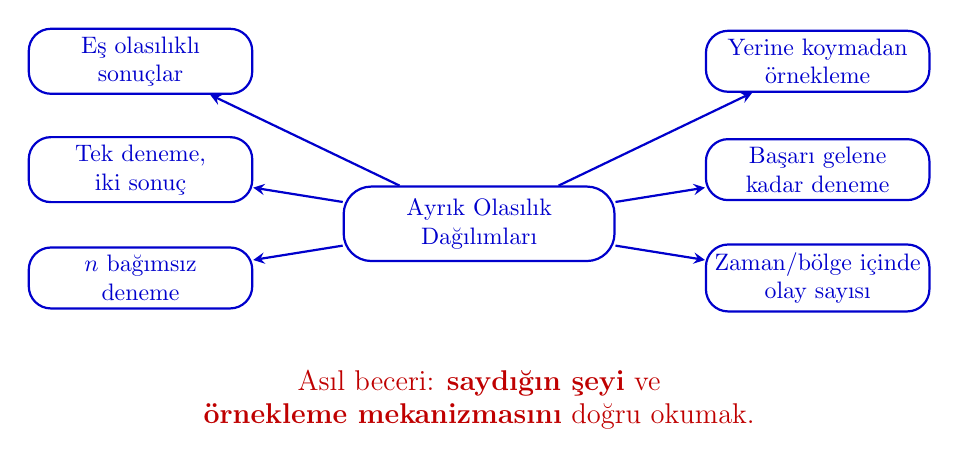
\begin{tikzpicture}[>=stealth, thick, scale=0.86, transform shape]
        \colorlet{myblue}{blue!80!black}
        \colorlet{myred}{red!75!black}

        \node[draw=myblue, rounded corners=10pt, minimum width=4.0cm, minimum height=1.1cm, text=myblue, align=center] (root) at (0,0) {Ayrık Olasılık\\Dağılımları};

        \node[draw=myblue, rounded corners=8pt, minimum width=3.3cm, minimum height=0.9cm, text=myblue, align=center] (uniform) at (-5,2.4) {Eş olasılıklı\\sonuçlar};
        \node[draw=myblue, rounded corners=8pt, minimum width=3.3cm, minimum height=0.9cm, text=myblue, align=center] (bern) at (-5,0.8) {Tek deneme,\\iki sonuç};
        \node[draw=myblue, rounded corners=8pt, minimum width=3.3cm, minimum height=0.9cm, text=myblue, align=center] (binom) at (-5,-0.8) {$n$ bağımsız\\deneme};
        \node[draw=myblue, rounded corners=8pt, minimum width=3.3cm, minimum height=0.9cm, text=myblue, align=center] (hyper) at (5,2.4) {Yerine koymadan\\örnekleme};
        \node[draw=myblue, rounded corners=8pt, minimum width=3.3cm, minimum height=0.9cm, text=myblue, align=center] (geom) at (5,0.8) {Başarı gelene\\kadar deneme};
        \node[draw=myblue, rounded corners=8pt, minimum width=3.3cm, minimum height=0.9cm, text=myblue, align=center] (pois) at (5,-0.8) {Zaman/bölge içinde\\olay sayısı};

        \draw[->, myblue] (root) -- (uniform);
        \draw[->, myblue] (root) -- (bern);
        \draw[->, myblue] (root) -- (binom);
        \draw[->, myblue] (root) -- (hyper);
        \draw[->, myblue] (root) -- (geom);
        \draw[->, myblue] (root) -- (pois);

        \node[text=myred, font=\large, align=center] at (0,-2.6) {Asıl beceri: \textbf{saydığın şeyi} ve\\ \textbf{örnekleme mekanizmasını} doğru okumak.};
    \end{tikzpicture}
\end{frame}

\begin{frame}{Neden Tek Tek PMF Yazmak Yetmez?}
    \small
    \begin{columns}[T]
        \begin{column}{0.48\textwidth}
            \begin{block}{Aynı tip davranış tekrar eder}
                \begin{itemize}
                    \item 10 üründe kusurlu sayısı
                    \item 5 kartta kırmızı sayısı
                    \item ilk başarılı çağrıya kadar deneme sayısı
                    \item 1 saatte gelen arıza kaydı sayısı
                \end{itemize}
            \end{block}

            \begin{itemize}
                \item Bu problemlerin hepsi ayrık değişken üretir.
                \item Ama PMF'nin \textbf{şekli} her seferinde sıfırdan kurulmaz.
            \end{itemize}
        \end{column}
        \begin{column}{0.48\textwidth}
            \begin{alertblock}{Dağılım ailesi ne kazandırır?}
                \begin{itemize}
                    \item Tek formülle birçok problemi çözme
                    \item Ortalama ve varyansı doğrudan okuma
                    \item Yaklaşım ve karşılaştırma yapabilme
                    \item Soru tipini daha hızlı tanıma
                \end{itemize}
            \end{alertblock}

            \vspace{0.2cm}
            \centering
            \textit{Bu yüzden önce ``hangi mekanizma?'' diye sorarız, sonra hesaplarız.}
        \end{column}
    \end{columns}
\end{frame}

\begin{frame}{Bu Haftanın Öğrenme Hedefleri}
    \small
    \begin{enumerate}
        \item Bir sayım problemini \textbf{uygun ayrık dağılım ailesine} eşleyebilmek.
        \item Bernoulli, binom, hipergeometrik, geometrik, negatif binom ve Poisson ailelerinin \textbf{koşullarını} ayırt edebilmek.
        \item Her aile için \textbf{olasılık fonksiyonu}, \textbf{ortalama} ve \textbf{varyans} ilişkisini okuyabilmek.
        \item ``Yerine koyma var mı?'', ``başarı sayısı mı bekleme sayısı mı?'', ``zaman aralığında olay mı?'' gibi model seçme sorularını doğru cevaplayabilmek.
        \item Bir probleme \textbf{yaklaşım} kullanmanın ne zaman makul olduğunu fark edebilmek.
    \end{enumerate}

    \begin{exampleblock}{Dersin tek cümlelik çıktısı}
        Saydığımız şeyin \textbf{nasıl üretildiğini} okuyarak doğru ayrık dağılımı seçebileceğiz.
    \end{exampleblock}
\end{frame}

\begin{frame}{Model Seçme Sorusu: Hangi Dağılım Neyi Sayar?}
    \scriptsize
    \begin{center}
        \resizebox{0.96\textwidth}{!}{
        \begin{tabular}{@{}lll@{}}
            \toprule
            \textbf{Problem cümlesi} & \textbf{Ana ipucu} & \textbf{Doğal aday} \\ \midrule
            Zarın üst yüzü & sonlu ve eş olasılıklı sonuçlar & ayrık uniform \\
            Tek ürün kusurlu mu? & iki sonuç, tek deneme & Bernoulli \\
            12 kartta kusurlu kart sayısı & sabit \(n\), bağımsız denemeler & binom \\
            5 kart çekip kırmızı sayısı & yerine koymadan seçim & hipergeometrik \\
            İlk başarılı çağrı kaçıncı denemede? & ilk başarıya kadar bekleme & geometrik \\
            3. başarılı test kaçıncı denemede? & \(k\). başarıya kadar bekleme & negatif binom \\
            1 saatte çağrı sayısı & zaman aralığında olay sayısı & Poisson \\ \bottomrule
        \end{tabular}}
    \end{center}

    \begin{alertblock}{Refleks}
        Önce şunu sorun:
        \textbf{``Başarı sayısı mı sayıyorum, yoksa bekleme sırası mı?''}
    \end{alertblock}
\end{frame}

\begin{frame}{Isınma: Ayrık Uniform ve Bernoulli Hatırlatması}
    \small
    \begin{columns}[T]
        \begin{column}{0.48\textwidth}
            \begin{block}{Ayrık uniform dağılım}
                Eğer \(m\) farklı sonuç \textbf{eş olasılıklı} ise
                \[
                P(X=x_i)=\frac{1}{m}, \qquad i=1,\dots,m.
                \]
                \textbf{Örnek:} adil bir zar için
                \[
                P(X=x)=\frac{1}{6}, \qquad x=1,2,3,4,5,6.
                \]
            \end{block}
        \end{column}
        \begin{column}{0.48\textwidth}
            \begin{block}{Bernoulli dağılımı}
                Tek denemede yalnızca iki sonuç vardır:
                başarı \(1\) ve başarısızlık \(0\).
                \[
                P(X=1)=p, \qquad P(X=0)=1-p.
                \]
                Bu, \textbf{binom dağılımının \(n=1\)} özel halidir.
            \end{block}

            \begin{alertblock}{Köprü}
                Bu iki kısa aile, birazdan göreceğimiz daha büyük ailelerin başlangıç sezgisini verir.
            \end{alertblock}
        \end{column}
    \end{columns}
\end{frame}

% ===================================================================
% SECTION 2
% ===================================================================
\section{Bernoulli Süreci ve Binom Dağılımı (Bölüm 5.2)}
\subsection{Bernoulli Süreci}

\begin{frame}{Bernoulli Süreci Nedir?}
    \small
    Bir deney aşağıdaki dört özelliği taşıyorsa \textbf{Bernoulli süreci} olarak okunur:
    \begin{enumerate}
        \item Deney tekrarlı yapılır.
        \item Her deneme yalnızca \textbf{başarı} veya \textbf{başarısızlık} üretir.
        \item Başarı olasılığı her denemede sabittir: \(p\).
        \item Denemeler birbirinden bağımsızdır.
    \end{enumerate}

    \begin{exampleblock}{Mühendislik okuması}
        Her kart için ``kusurlu / kusursuz'', her modem için ``bağlandı / bağlanmadı'', her test için ``geçti / kaldı'' dili Bernoulli süreci kurmaya adaydır.
    \end{exampleblock}
\end{frame}

\begin{frame}{Bernoulli Değişkeni: 0--1 Dili}
    \small
    \begin{block}{Tanım}
        Tek bir denemede
        \[
        X=
        \begin{cases}
        1, & \text{başarı ise},\\
        0, & \text{başarısızlık ise}.
        \end{cases}
        \]
    \end{block}

    \begin{itemize}
        \item Bernoulli değişkeni \textbf{durumu sayıya çevirir}.
        \item Birden çok Bernoulli değişkeninin toplamı, toplam başarı sayısını verir.
        \item Bu yüzden binom dağılımını \textbf{başarı göstergelerinin toplamı} gibi okuyabiliriz.
    \end{itemize}

    \[
    X_1+X_2+\cdots+X_n = \text{toplam başarı sayısı}.
    \]
\end{frame}

\subsection{Binom Dağılımı}

\begin{frame}{Binom Dağılımı: Saydığımız Başarı Sayısı}
    \small
    \begin{block}{Tanım}
        \(n\) bağımsız Bernoulli denemesinde başarı olasılığı \(p\) ise,
        başarı sayısı \(X\) için
        \[
        X \sim \mathrm{Bin}(n,p)
        \]
        yazılır.
    \end{block}

    \begin{itemize}
        \item \(X\), \textbf{kaç başarı geldiğini} sayar.
        \item Değer kümesi
        \[
        X=\{0,1,2,\dots,n\}
        \]
        olur.
        \item Her denemede olasılık sabit değilse veya bağımsızlık bozulursa binom modeli zayıflar.
    \end{itemize}
\end{frame}

\begin{frame}{Binom Formülü Neden Böyle Görünür?}
    \small
    Tam \(x\) başarı gelmesi için iki şey gerekir:
    \begin{enumerate}
        \item Belirli bir sıranın olasılığı: \(p^x(1-p)^{n-x}\)
        \item Bu sıranın kaç farklı şekilde oluşabileceği:
        \[
        \binom{n}{x}
        \]
    \end{enumerate}

    \begin{block}{Binom olasılık fonksiyonu}
        \[
        b(x;n,p)=\binom{n}{x}p^x(1-p)^{n-x},
        \qquad x=0,1,\dots,n.
        \]
    \end{block}

    \begin{alertblock}{Okuma}
        \(\binom{n}{x}\) düzen sayısını, \(p^x(1-p)^{n-x}\) ise her düzenin ağırlığını taşır.
    \end{alertblock}
\end{frame}

\begin{frame}{Örnek 1: Şok Testini Geçen Parça Sayısı}
    \small
    Bir bileşenin şok testini geçme olasılığı \(p=0.75\) olsun. Sıradaki \(4\) bileşenden tam \(2\) tanesinin testi geçme olasılığı nedir?

    \vspace{0.2cm}
    \begin{block}{Model}
        \[
        X \sim \mathrm{Bin}(4,0.75), \qquad P(X=2)=\binom{4}{2}(0.75)^2(0.25)^2.
        \]
    \end{block}

    \[
    P(X=2)=6(0.5625)(0.0625)=0.2109.
    \]

    \begin{exampleblock}{Yorum}
        Tam iki başarılı bileşen görme olasılığı yaklaşık \(\%21.1\)'dir.
    \end{exampleblock}
\end{frame}

\begin{frame}{Örnek 2: Kuyu Örneklemesinde Tam 3 Kirli Kuyu}
    \small
    Bir bölgede kuyuların \(\%30\)'unun kirli olduğu biliniyor. Rastgele seçilen \(10\) kuyudan tam \(3\)'ünün kirli olma olasılığını bulun.

    \vspace{0.2cm}
    \[
    X \sim \mathrm{Bin}(10,0.30)
    \]
    \[
    P(X=3)=\binom{10}{3}(0.30)^3(0.70)^7.
    \]
    \[
    P(X=3)=120(0.027)(0.0823543)\approx 0.2668.
    \]

    \begin{alertblock}{Mesaj}
        ``Kuyu sayısı sabit, her kuyu için kirli/temiz ayrımı var, oran sabit'' olduğu için binom doğrudur.
    \end{alertblock}
\end{frame}

\begin{frame}{Ortalama ve Varyans: Binomun Merkezi ve Yayılımı}
    \small
    \(X \sim \mathrm{Bin}(n,p)\) için
    \[
    \mu = E(X)=np, \qquad \sigma^2=\mathrm{Var}(X)=np(1-p).
    \]

    \begin{columns}[T]
        \begin{column}{0.48\textwidth}
            \begin{block}{Sezgi}
                \begin{itemize}
                    \item \(np\): beklenen başarı sayısı
                    \item \(1-p\): başarısızlık payı
                    \item yayılım, hem başarı hem başarısızlık olasılığına bağlı
                \end{itemize}
            \end{block}
        \end{column}
        \begin{column}{0.48\textwidth}
            \begin{exampleblock}{Kısa örnek}
                Eğer \(n=15\) ve \(p=0.4\) ise
                \[
                E(X)=15(0.4)=6,
                \]
                \[
                \mathrm{Var}(X)=15(0.4)(0.6)=3.6.
                \]
            \end{exampleblock}
        \end{column}
    \end{columns}
\end{frame}

\begin{frame}{Binom Sorularında Kontrol Listesi}
    \small
    \begin{enumerate}
        \item Deneme sayısı sabit mi?
        \item Her denemede yalnızca iki sonuç mu var?
        \item Başarı olasılığı sabit mi?
        \item Denemeler bağımsız mı?
        \item Aradığımız şey \textbf{başarı sayısı} mı?
    \end{enumerate}

    \begin{alertblock}{Sık hata}
        ``Örneklem büyüklüğü sabit'' görmek tek başına yetmez. Eğer seçim \textbf{yerine koymadan} yapılıyorsa hipergeometrik düşünmek gerekir.
    \end{alertblock}
\end{frame}

\subsection{Pekiştirme Soruları}

\begin{frame}{Soru 1: Lehim Hattında Kusurlu Kart Sayısı}
    \small
    Bir elektronik kart hattında her kartın kusurlu çıkma olasılığı \(0.08\) olarak modelleniyor ve kartlar bağımsız kabul ediliyor. Rastgele seçilen \(12\) kart için:

    \begin{enumerate}
        \item[(a)] Tam \(2\) kartın kusurlu olma olasılığını bulun.
        \item[(b)] En fazla \(2\) kartın kusurlu olma olasılığını bulun.
    \end{enumerate}

    \begin{block}{İpucu}
        Bu bir \textbf{başarı sayısı} problemidir; burada başarıyı ``kart kusurlu'' diye okuyun.
    \end{block}
\end{frame}

\begin{frame}{Soru 1: Çözüm İçin Durak}
    \color{red!70!black}
    \small
    \[
    X \sim \mathrm{Bin}(12,0.08)
    \]
    \[
    P(X=2)=\binom{12}{2}(0.08)^2(0.92)^{10}
    \]
    \[
    P(X\le 2)=P(X=0)+P(X=1)+P(X=2)
    \]

    \begin{center}
        \textit{Önce modeli ve parametreleri doğrulayın, sonra olasılıkları yazın.}
    \end{center}
\end{frame}

\begin{frame}{Soru 1: Çözüm}
    \small
    \[
    P(X=2)=\binom{12}{2}(0.08)^2(0.92)^{10}\approx 0.1835.
    \]

    \[
    P(X\le 2)=\sum_{x=0}^{2}\binom{12}{x}(0.08)^x(0.92)^{12-x}\approx 0.9348.
    \]

    \begin{exampleblock}{Yorum}
        Süreç kusur oranı düşük olduğu için \(12\) kart içinde \(2\) veya daha az kusurlu kart görme olasılığı oldukça yüksektir.
    \end{exampleblock}
\end{frame}

\begin{frame}{Soru 2: Bernoulli mi, Binom mu?}
    \small
    Aşağıdaki değişkenleri uygun dağılımla eşleyin:
    \begin{enumerate}
        \item[(i)] Tek bir sensörün kalibrasyonu geçip geçmediği
        \item[(ii)] Aynı tip \(20\) sensörden kalibrasyonu geçenlerin sayısı
    \end{enumerate}

    \begin{alertblock}{Düşünme noktası}
        İkisi de iki sonuçlu olay dili kullanıyor. Farkı yaratan şey \textbf{kaç deneme saydığımızdır}.
    \end{alertblock}
\end{frame}

\begin{frame}{Soru 2: Çözüm}
    \small
    \begin{itemize}
        \item[(i)] Tek sensör: \textbf{Bernoulli}. Çünkü yalnızca bir deneme var.
        \item[(ii)] \(20\) sensörde geçen sayısı: \textbf{Binom}. Çünkü sabit sayıda bağımsız denemede başarı sayısı aranıyor.
    \end{itemize}

    \begin{block}{Kural}
        \[
        \text{Bernoulli} = \text{Binomun } n=1 \text{ özel hali.}
        \]
    \end{block}
\end{frame}

% ===================================================================
% SECTION 3
% ===================================================================
\section{Çok Kategorili Sayım ve Multinomial Uzantısı}
\subsection{Binomun Genişlemesi}

\begin{frame}{İki Sonuç Yetmezse: Multinomial Fikir}
    \small
    Binom dağılımında her denemede yalnızca iki sonuç vardı: başarı veya başarısızlık.

    \vspace{0.2cm}
    Peki her denemede \(k\) farklı sonuç varsa ne olur?

    \begin{itemize}
        \item trafik yönü: kuzey, güney, doğu, batı
        \item kalite sınıfı: A, B, C
        \item ulaşım türü: kara, hava, demir, deniz
    \end{itemize}

    \begin{alertblock}{Köprü}
        Bu durumda başarı sayısı değil, \textbf{her kategoride kaç gözlem geldiğini} birlikte sayarız.
    \end{alertblock}
\end{frame}

\begin{frame}{Multinomial Dağılım: Genel Formül}
    \small
    Her denemede \(k\) kategori olsun ve olasılıklar
    \[
    p_1,p_2,\dots,p_k, \qquad p_1+\cdots+p_k=1.
    \]
    \(n\) denemede \(x_1,\dots,x_k\) sayıları gözlenirse
    \[
    x_1+\cdots+x_k=n
    \]
    ve olasılık
    \[
    P(X_1=x_1,\dots,X_k=x_k)=
    \frac{n!}{x_1!\cdots x_k!}p_1^{x_1}\cdots p_k^{x_k}.
    \]

    \begin{block}{Özel durum}
        \(k=2\) olduğunda multinomial, binom dağılımına geri döner.
    \end{block}
\end{frame}

\begin{frame}{Uygulama: Kavşakta Yön Dağılımı}
    \small
    Bir kavşakta gelen araçların yön oranları sırasıyla
    \[
    p_{\text{kuzey}}=0.15,\quad p_{\text{güney}}=0.25,\quad p_{\text{doğu}}=0.60
    \]
    olsun. \(12\) araç içinde \(2\) kuzey, \(3\) güney ve \(7\) doğu yönlü araç görme olasılığı:
    \[
    \frac{12!}{2!3!7!}(0.15)^2(0.25)^3(0.60)^7.
    \]

    \[
    P\approx 0.0779.
    \]

    \begin{exampleblock}{Yorum}
        Burada binom yeterli değildir; çünkü tek başarı kategorisi değil, \textbf{üçlü dağılım profili} önemlidir.
    \end{exampleblock}
\end{frame}

\begin{frame}{Binom ile Multinomial Arasındaki Köprü}
    \small
    \begin{columns}[T]
        \begin{column}{0.48\textwidth}
            \begin{block}{Binom}
                \begin{itemize}
                    \item İki kategori
                    \item Tek başarı sayısı
                    \item Parametreler: \(n,p\)
                \end{itemize}
            \end{block}
        \end{column}
        \begin{column}{0.48\textwidth}
            \begin{block}{Multinomial}
                \begin{itemize}
                    \item Birden çok kategori
                    \item Kategori sayılarının tamamı
                    \item Parametreler: \(n,p_1,\dots,p_k\)
                \end{itemize}
            \end{block}
        \end{column}
    \end{columns}

    \begin{alertblock}{Karar}
        ``Kaç başarı?'' sorusu varsa binom; ``hangi kategoriden kaç tane?'' sorusu varsa multinomial düşünülür.
    \end{alertblock}
\end{frame}

\subsection{Pekiştirme Sorusu}

\begin{frame}{Soru 3: Kalite Sınıfları Dağılımı}
    \small
    Bir üretim hattında ürünler A, B ve C kalite sınıfına ayrılıyor. Olasılıklar sırasıyla \(0.50\), \(0.30\) ve \(0.20\). Rastgele seçilen \(8\) ürün içinde \(4\) A, \(3\) B ve \(1\) C ürünü bulunma olasılığı nedir?

    \begin{block}{İpucu}
        Tek bir başarı saymıyoruz; üç kategorinin dağılımını birlikte sayıyoruz.
    \end{block}
\end{frame}

\begin{frame}{Soru 3: Çözüm}
    \small
    \[
    P=\frac{8!}{4!3!1!}(0.50)^4(0.30)^3(0.20)^1.
    \]

    \[
    P=280(0.0625)(0.027)(0.20)\approx 0.0945.
    \]

    \begin{exampleblock}{Yorum}
        Multinomial yapı, kalite dağılımı gibi çok kategorili üretim tablolarını doğal biçimde modellemek için kullanılır.
    \end{exampleblock}
\end{frame}

% ===================================================================
% SECTION 4
% ===================================================================
\section{Hipergeometrik Dağılım (Bölüm 5.3)}
\subsection{Yerine Koymadan Örnekleme}

\begin{frame}{Yerine Koymadan Seçim: Neden Binom Yetmez?}
    \small
    Eğer örnekleme sırasında seçilen eleman tekrar havuza dönmüyorsa, her çekişten sonra olasılıklar değişir.

    \begin{itemize}
        \item kart destesi
        \item üretim partisinden örnek alma
        \item stoktan parça çekme
    \end{itemize}

    \begin{alertblock}{Kritik fark}
        Binom için gerekli olan \textbf{bağımsızlık} artık yoktur. Çünkü ilk çekiliş ikinci çekilişi etkiler.
    \end{alertblock}
\end{frame}

\begin{frame}{Kartlardan Lotlara: Hipergeometrik Sezgi}
    \small
    \(52\) karttan yerine koymadan \(5\) kart çekip tam \(3\) kırmızı kart gelmesini düşünelim.

    \[
    \frac{\binom{26}{3}\binom{26}{2}}{\binom{52}{5}}
    \]
    ifadesi
    \begin{itemize}
        \item payda: tüm \(5\) kartlık seçimleri,
        \item pay: \(3\) kırmızı ve \(2\) siyah veren seçimleri
    \end{itemize}
    sayar.

    \begin{exampleblock}{Mühendislik yorumu}
        Aynı mantık kalite kontrolde ``lot içindeki kusurlular'' ve ``örnekleme içinde yakalanan kusurlular'' için de geçerlidir.
    \end{exampleblock}
\end{frame}

\begin{frame}{Hipergeometrik Dağılımın Formülü}
    \small
    Toplam \(N\) eleman olsun. Bunların \(k\) tanesi başarı, \(N-k\) tanesi başarısızlık olsun. Yerine koymadan seçilen \(n\) eleman içinde tam \(x\) başarı gelme olasılığı:
    \[
    h(x;N,n,k)=
    \frac{\binom{k}{x}\binom{N-k}{n-x}}{\binom{N}{n}}.
    \]

    \begin{block}{Değer kümesi}
        \(x\), hem başarı sayısı sınırını hem de örneklem büyüklüğünü aşamaz.
    \end{block}

    \begin{alertblock}{Ana fikir}
        Hipergeometrik dağılım, \textbf{sonlu popülasyondan yerine koymadan örnek alma} problemidir.
    \end{alertblock}
\end{frame}

\begin{frame}{Örnek 4: 10 Parçalık Lottaki Kabul Riski}
    \small
    Bir üretici, \(10\) parçalık bir lotta en fazla \(1\) kusur olmasını kabul edilebilir sayıyor. Kalite kontrol planı, lottan rastgele \(3\) parça seçip hepsi sağlam ise lotu kabul ediyor. Lotta aslında \(2\) kusurlu parça varsa, planın lotu yanlış kabul etme olasılığı nedir?

    \[
    X \sim \text{Hipergeom}(N=10,n=3,k=2)
    \]
    \[
    P(X=0)=\frac{\binom{2}{0}\binom{8}{3}}{\binom{10}{3}}=\frac{56}{120}=0.4667.
    \]

    \begin{alertblock}{Yorum}
        Gerçekte kabul edilmemesi gereken lot, yaklaşık \(\%46.7\) olasılıkla kabul ediliyor. Plan zayıf.
    \end{alertblock}
\end{frame}

\begin{frame}{Kabul Örneklemesinde Sonuç Ne Söyler?}
    \small
    \begin{itemize}
        \item Lot küçükse ve örneklem lotun kayda değer kısmını kapsıyorsa, \textbf{yerine koymadan örnekleme etkisi} büyür.
        \item Bu durumda binom kullanmak risklidir; çünkü kusur olasılığı her çekimde sabit değildir.
        \item Hipergeometrik model, örnekleme planının \textbf{yanlış kabul / yanlış ret} davranışını daha doğru okur.
    \end{itemize}

    \begin{block}{Pratik soru}
        Örneklem büyüklüğü büyüdükçe lot içindeki gizli kusur yapısı daha hızlı ``tükenir''. Bu etki binomda görünmez, hipergeometrikte görünür.
    \end{block}
\end{frame}

\begin{frame}{Ortalama ve Varyans: Sonlu Popülasyon Düzeltmesi}
    \small
    \(X \sim \text{Hipergeom}(N,n,k)\) için
    \[
    E(X)=n\frac{k}{N}
    \]
    ve
    \[
    \mathrm{Var}(X)=n\frac{k}{N}\left(1-\frac{k}{N}\right)\frac{N-n}{N-1}.
    \]

    \begin{alertblock}{Neden ekstra çarpan var?}
        \[
        \frac{N-n}{N-1}
        \]
        terimi, \textbf{yerine koymadan örnekleme} yüzünden oluşan sonlu popülasyon düzeltmesidir.
    \end{alertblock}
\end{frame}

\begin{frame}{Binom mu Hipergeometrik mi?}
    \small
    \begin{columns}[T]
        \begin{column}{0.48\textwidth}
            \begin{block}{Binom}
                \begin{itemize}
                    \item bağımsız denemeler
                    \item sabit \(p\)
                    \item gerekirse yerine koyma
                \end{itemize}
            \end{block}
        \end{column}
        \begin{column}{0.48\textwidth}
            \begin{block}{Hipergeometrik}
                \begin{itemize}
                    \item sonlu popülasyon
                    \item yerine koymadan seçim
                    \item çekişler birbirini etkiler
                \end{itemize}
            \end{block}
        \end{column}
    \end{columns}

    \begin{exampleblock}{Kısa karar}
        ``Lot içinden örnek alıyorum'' diyorsanız önce hipergeometrik düşünün; sonra gerekirse binom yaklaşıklığını tartışın.
    \end{exampleblock}
\end{frame}

\begin{frame}{Büyük Popülasyonda Binom Yaklaşımı}
    \small
    Eğer popülasyon çok büyük ve örneklem göreli olarak küçükse, hipergeometrik dağılım binoma yaklaşır.

    \[
    p \approx \frac{k}{N}
    \]
    seçilerek
    \[
    \text{Hipergeom}(N,n,k) \approx \mathrm{Bin}\left(n,\frac{k}{N}\right)
    \]
    kullanılabilir.

    \begin{exampleblock}{Örnek}
        \(5000\) lastikten \(50\) tanesi kusurluysa ve yalnızca \(4\) lastik seçiyorsanız,
        \[
        P(X=0)\approx (0.99)^4 \approx 0.9606
        \]
        değeri hipergeometrik sonuca çok yakındır.
    \end{exampleblock}
\end{frame}

\subsection{Pekiştirme Sorusu}

\begin{frame}{Soru 4: 40 Parçalık Partide Tam 1 Kusurlu}
    \small
    \(40\) parçalık bir partide \(3\) kusurlu parça bulunduğu biliniyor. Partiden yerine koymadan \(5\) parça seçiliyor. Seçilen örnek içinde tam \(1\) kusurlu parça bulunma olasılığı nedir?

    \begin{block}{İpucu}
        Burada başarıyı ``kusurlu parça seçmek'' olarak okuyun.
    \end{block}
\end{frame}

\begin{frame}{Soru 4: Çözüm İçin Durak}
    \color{red!70!black}
    \small
    \[
    X \sim \text{Hipergeom}(N=40,n=5,k=3)
    \]
    \[
    P(X=1)=\frac{\binom{3}{1}\binom{37}{4}}{\binom{40}{5}}
    \]

    \begin{center}
        \textit{Payda tüm 5'li örnekleri, pay ise 1 kusurlu + 4 sağlam örnekleri sayar.}
    \end{center}
\end{frame}

\begin{frame}{Soru 4: Çözüm}
    \small
    \[
    P(X=1)=\frac{\binom{3}{1}\binom{37}{4}}{\binom{40}{5}}\approx 0.3011.
    \]

    \begin{exampleblock}{Yorum}
        Örnekte tam bir kusur yakalama olasılığı yaklaşık \(\%30.1\)'dir. Bu sonuç, örnekleme planının kusurlu lotu ne kadar görünür kıldığına dair fikir verir.
    \end{exampleblock}
\end{frame}

% ===================================================================
% SECTION 5
% ===================================================================
\section{Geometrik ve Negatif Binom Dağılımlar (Bölüm 5.4)}
\subsection{Bekleme Sayısı Problemleri}

\begin{frame}{Başarı Gelene Kadar Beklemek}
    \small
    Bazı problemler ``kaç başarı geldi?'' diye sormaz; bunun yerine
    \textbf{başarı gelene kadar kaç deneme gerektiğini} sorar.

    \begin{itemize}
        \item ilk bağlantının kaçıncı denemede kurulacağı
        \item ilk kusurlu ürünün kaçıncı kontrolde bulunacağı
        \item üçüncü başarılı testin kaçıncı denemede geleceği
    \end{itemize}

    \begin{alertblock}{Fark}
        Artık rastgele değişkenin anlamı \textbf{başarı sayısı} değil, \textbf{deneme sırası}dır.
    \end{alertblock}
\end{frame}

\begin{frame}{Negatif Binom Dağılımı: \(k\). Başarı Ne Zaman?}
    \small
    Negatif binom deneyinde
    \begin{itemize}
        \item denemeler bağımsızdır,
        \item her denemede başarı olasılığı \(p\) sabittir,
        \item süreç, \textbf{\(k\). başarı} elde edilince durur.
    \end{itemize}

    \begin{block}{Rastgele değişken}
        \(X\): \(k\). başarının geldiği deneme numarası
    \end{block}

    \[
    X = k,k+1,k+2,\dots
    \]
\end{frame}

\begin{frame}{Negatif Binom Formülü}
    \small
    \(k\). başarının tam \(x\). denemede gelmesi için
    \begin{itemize}
        \item ilk \(x-1\) denemede tam \(k-1\) başarı,
        \item son denemede başarı
    \end{itemize}
    gerekir.

    \begin{block}{Olasılık fonksiyonu}
        \[
        b^{\ast}(x;k,p)=\binom{x-1}{k-1}p^k(1-p)^{x-k},
        \qquad x=k,k+1,\dots
        \]
    \end{block}
\end{frame}

\begin{frame}{Örnek 5: Dördüncü Başarılı Modül 6. Denemede}
    \small
    Bir modülün testi geçme olasılığı \(p=0.60\) olsun. Dördüncü başarılı modülün tam \(6\). denemede görülme olasılığı:
    \[
    P(X=6)=\binom{5}{3}(0.60)^4(0.40)^2.
    \]

    \[
    P(X=6)=10(0.1296)(0.16)=0.20736.
    \]

    \begin{exampleblock}{Yorum}
        İlk \(5\) denemede \(3\) başarı, son denemede de başarı gerekir. Son deneme zorunlu olarak başarıdır.
    \end{exampleblock}
\end{frame}

\begin{frame}{Geometrik Dağılım: İlk Başarı}
    \small
    Negatif binomun \(k=1\) özel haline \textbf{geometrik dağılım} denir.

    \begin{block}{Rastgele değişken}
        \(X\): ilk başarının geldiği deneme numarası
    \end{block}

    \[
    g(x;p)=p(1-p)^{x-1}, \qquad x=1,2,3,\dots
    \]

    \begin{alertblock}{Yorum}
        İlk \(x-1\) denemede başarısızlık, \(x\). denemede başarı gerekir.
    \end{alertblock}
\end{frame}

\begin{frame}{Örnek 6: Beşinci Kontrolde İlk Kusur}
    \small
    Bir üretim sürecinde her ürünün kusurlu olma olasılığı \(0.01\) olsun. İncelenen \(5\). ürünün ilk kusurlu ürün olma olasılığı nedir?

    \[
    X \sim \text{Geom}(0.01)
    \]
    \[
    P(X=5)=0.01(0.99)^4\approx 0.0096.
    \]

    \begin{exampleblock}{Yorum}
        İlk \(4\) ürün sağlam, \(5\). ürün kusurlu olmalıdır.
    \end{exampleblock}
\end{frame}

\begin{frame}{Geometrikte Ortalama ve Varyans}
    \small
    Geometrik dağılım için
    \[
    E(X)=\frac{1}{p}, \qquad \mathrm{Var}(X)=\frac{1-p}{p^2}.
    \]

    \begin{columns}[T]
        \begin{column}{0.48\textwidth}
            \begin{block}{Sezgi}
                \begin{itemize}
                    \item başarı zorlaştıkça \(p\) küçülür,
                    \item beklenen bekleme süresi büyür,
                    \item belirsizlik de artar.
                \end{itemize}
            \end{block}
        \end{column}
        \begin{column}{0.48\textwidth}
            \begin{exampleblock}{Bağlantı örneği}
                Eğer \(p=0.05\) ise
                \[
                E(X)=20
                \]
                deneme gerekir.
            \end{exampleblock}
        \end{column}
    \end{columns}
\end{frame}

\begin{frame}{Geometrik ile Negatif Binom Nasıl Ayrılır?}
    \small
    \begin{center}
        \begin{tabular}{@{}lll@{}}
            \toprule
            \textbf{Dağılım} & \textbf{Ne sayar?} & \textbf{Durma koşulu} \\ \midrule
            Geometrik & ilk başarının geldiği deneme & \(1\). başarı \\
            Negatif binom & \(k\). başarının geldiği deneme & \(k\). başarı \\ \bottomrule
        \end{tabular}
    \end{center}

    \begin{alertblock}{Sık hata}
        Aynı veriyi bazen ``kaç başarı?'' bazen de ``kaçıncı denemede başarı?'' diye okumak mümkündür; bu iki okuma farklı dağılımlar üretir.
    \end{alertblock}
\end{frame}

\subsection{Pekiştirme Soruları}

\begin{frame}{Soru 5: Sensör Kalibrasyonunda İlk Başarı}
    \small
    Bir sensörün tek denemede kalibrasyonu geçme olasılığı \(0.20\) olsun. İlk başarılı kalibrasyonun tam \(4\). denemede görülme olasılığını bulun.

    \begin{block}{İpucu}
        Burada \textbf{ilk başarı} aranıyor.
    \end{block}
\end{frame}

\begin{frame}{Soru 5: Çözüm İçin Durak}
    \color{red!70!black}
    \small
    \[
    X \sim \text{Geom}(0.20)
    \]
    \[
    P(X=4)=0.20(0.80)^3
    \]

    \begin{center}
        \textit{İlk üç deneme başarısız, dördüncü deneme başarılıdır.}
    \end{center}
\end{frame}

\begin{frame}{Soru 5: Çözüm}
    \small
    \[
    P(X=4)=0.20(0.512)=0.1024.
    \]

    \begin{exampleblock}{Yorum}
        İlk başarılı kalibrasyonun \(4\). denemede gelme olasılığı yaklaşık \(\%10.24\)'tür.
    \end{exampleblock}
\end{frame}

\begin{frame}{Soru 6: Üçüncü Başarı 5. Denemede}
    \small
    Bir test protokolünde tek denemede başarı olasılığı \(0.70\) olsun. Üçüncü başarının tam \(5\). denemede gelme olasılığı nedir?

    \begin{block}{İpucu}
        Bu kez ilk başarı değil, \textbf{üçüncü başarı} isteniyor.
    \end{block}
\end{frame}

\begin{frame}{Soru 6: Çözüm}
    \small
    \[
    P(X=5)=\binom{4}{2}(0.70)^3(0.30)^2.
    \]

    \[
    P(X=5)=6(0.343)(0.09)\approx 0.1852.
    \]

    \begin{exampleblock}{Yorum}
        İlk \(4\) denemede tam \(2\) başarı olmalı, \(5\). denemede üçüncü başarı gelmelidir.
    \end{exampleblock}
\end{frame}

% ===================================================================
% SECTION 6
% ===================================================================
\section{Poisson Dağılımı ve Poisson Süreci (Bölüm 5.5)}
\subsection{Zaman ve Bölge İçinde Olay Sayısı}

\begin{frame}{Zaman ve Bölge Üzerinde Olay Saymak}
    \small
    Poisson modeli, belirli bir \textbf{zaman aralığında} ya da \textbf{uzay/bölge içinde} kaç olay gerçekleştiğini sayar.

    \begin{itemize}
        \item bir saatte gelen çağrı sayısı
        \item bir sayfadaki yazım hatası sayısı
        \item bir levhadaki hava kabarcığı sayısı
        \item bir dakikadaki sensör alarmı sayısı
    \end{itemize}

    \begin{alertblock}{Fark}
        Burada denemeleri tek tek saymıyoruz; \textbf{bir aralık içindeki olay sayısını} sayıyoruz.
    \end{alertblock}
\end{frame}

\begin{frame}{Poisson Sürecinin Üç Özelliği}
    \small
    \begin{enumerate}
        \item Ayrık zaman aralıkları veya ayrık bölgelerdeki olay sayıları bağımsızdır.
        \item Çok kısa bir aralıkta bir olay gelme olasılığı, aralığın uzunluğu ile orantılıdır.
        \item Çok kısa bir aralıkta birden fazla olay gelme olasılığı ihmal edilebilir.
    \end{enumerate}

    \begin{block}{Mühendislik yorumu}
        Olaylar seyrek ve birbirinden bağımsız görünüyorsa Poisson düşünmek makuldür.
    \end{block}
\end{frame}

\begin{frame}{Poisson Dağılımı: Parametre ve Formül}
    \small
    Olayların birim zamanda ortalama geliş hızı \(\lambda\) ve incelenen aralık \(t\) ise
    \[
    \mu=\lambda t
    \]
    beklenen olay sayısıdır.

    \begin{block}{Olasılık fonksiyonu}
        \[
        p(x;\mu)=e^{-\mu}\frac{\mu^x}{x!},
        \qquad x=0,1,2,\dots
        \]
    \end{block}

    \begin{alertblock}{Okuma}
        Poisson dağılımında temel parametre, aralık başına \textbf{ortalama olay sayısıdır}.
    \end{alertblock}
\end{frame}

\begin{frame}{Örnek 7: Bir Milisaniyedeki Parçacık Sayısı}
    \small
    Bir laboratuvar sayacından \(1\) milisaniyede ortalama \(4\) parçacık geçiyor. Tam \(6\) parçacık geçme olasılığı nedir?

    \[
    X \sim \text{Pois}(\mu=4)
    \]
    \[
    P(X=6)=e^{-4}\frac{4^6}{6!}\approx 0.1042.
    \]

    \begin{exampleblock}{Yorum}
        Ortalama \(4\) olmasına rağmen tam \(6\) olay görme olasılığı yaklaşık \(\%10.4\)'tür.
    \end{exampleblock}
\end{frame}

\begin{frame}{Ortalama ve Varyans Neden Aynı?}
    \small
    Poisson dağılımı için
    \[
    E(X)=\mu, \qquad \mathrm{Var}(X)=\mu.
    \]

    \begin{block}{Bu ne anlatır?}
        Olay yoğunluğu arttıkça hem merkez hem de yayılım aynı büyüklük sırasıyla artar.
    \end{block}

    \begin{exampleblock}{Kısa örnek}
        Saatte ortalama \(3\) arıza kaydı varsa
        \[
        E(X)=3, \qquad \mathrm{Var}(X)=3.
        \]
    \end{exampleblock}
\end{frame}

\begin{frame}{Poisson Şekli: Ortalama Büyüdükçe Ne Olur?}
    \small
    \begin{itemize}
        \item \(\mu\) çok küçükken dağılım \(0\) etrafında yoğunlaşır.
        \item \(\mu\) büyüdükçe dağılım daha geniş ve daha simetrik görünür.
        \item Bu yüzden Poisson şekli, olay yoğunluğunun büyüklüğüne duyarlıdır.
    \end{itemize}

    \begin{alertblock}{Sezgi}
        Seyrek olaylar sağa çarpık görünür; ortalama yükseldikçe biçim daha dengeli hale gelir.
    \end{alertblock}
\end{frame}

\begin{frame}{Binomdan Poisson'a Yaklaşım}
    \small
    Eğer
    \[
    n \text{ büyük}, \qquad p \text{ küçük}
    \]
    ise
    \[
    \mathrm{Bin}(n,p)\approx \mathrm{Pois}(\mu=np)
    \]
    yaklaşımı kullanılabilir.

    \begin{block}{Ne zaman işe yarar?}
        Büyük örneklemde nadir kusur, nadir kaza, nadir arıza gibi problemler için.
    \end{block}
\end{frame}

\begin{frame}{Örnek 8: 400 Günde Kaza Sayısı}
    \small
    Bir tesiste herhangi bir günde kaza olma olasılığı \(0.005\) ve günler bağımsız kabul edilsin. \(400\) günlük dönemde:
    \begin{enumerate}
        \item[(a)] tam \(1\) kaza günü,
        \item[(b)] en fazla \(3\) kaza günü
    \end{enumerate}
    olma olasılıklarını Poisson yaklaşımıyla bulun.

    \[
    \mu=np=400(0.005)=2.
    \]

    \[
    P(X=1)=e^{-2}\frac{2^1}{1!}\approx 0.2707,
    \]
    \[
    P(X\le 3)\approx 0.8571.
    \]
\end{frame}

\begin{frame}{Örnek 9: 8000 Cam Üründe Kusur Sayısı}
    \small
    Cam üretiminde her ürünün kusurlu olma olasılığı \(0.001\) olsun. \(8000\) ürün içinde \(7\)'den az kusurlu ürün bulunma olasılığı nedir?

    \[
    \mu=np=8000(0.001)=8.
    \]

    \[
    P(X<7)=\sum_{x=0}^{6} e^{-8}\frac{8^x}{x!}\approx 0.3134.
    \]

    \begin{exampleblock}{Yorum}
        Büyük \(n\), küçük \(p\) olduğu için binom yerine Poisson yaklaşımı rahatlıkla kullanılabilir.
    \end{exampleblock}
\end{frame}

\begin{frame}{Poisson Sorularında Sık Hata}
    \small
    \begin{enumerate}
        \item ``Ortalama sabit'' varsayımını sorgulamadan kabul etmek
        \item yoğun saat / sakin saat farkını yok saymak
        \item bağımsız olmayan kümelenmiş olayları Poisson sanmak
        \item nadir olmayan olaylarda Poisson yaklaşımını ezbere kullanmak
    \end{enumerate}

    \begin{alertblock}{Kitaptaki uyarı}
        Tarihsel ortalama ile bugünkü süreç aynı değilse, Poisson hesabı sayısal olarak doğru görünse bile model olarak yanlış olabilir.
    \end{alertblock}
\end{frame}

\subsection{Pekiştirme Sorusu}

\begin{frame}{Soru 7: Saatlik Arıza Kaydı Sayısı}
    \small
    Bir sunucu odasında saatte ortalama \(3\) arıza kaydı oluştuğu gözleniyor. Bir saatte
    \begin{enumerate}
        \item[(a)] tam \(5\) kayıt,
        \item[(b)] en fazla \(2\) kayıt
    \end{enumerate}
    oluşma olasılıklarını bulun.
\end{frame}

\begin{frame}{Soru 7: Çözüm İçin Durak}
    \color{red!70!black}
    \small
    \[
    X \sim \text{Pois}(\mu=3)
    \]
    \[
    P(X=5)=e^{-3}\frac{3^5}{5!}
    \]
    \[
    P(X\le 2)=\sum_{x=0}^{2} e^{-3}\frac{3^x}{x!}
    \]
\end{frame}

\begin{frame}{Soru 7: Çözüm}
    \small
    \[
    P(X=5)=e^{-3}\frac{3^5}{5!}\approx 0.1008.
    \]

    \[
    P(X\le 2)=\sum_{x=0}^{2} e^{-3}\frac{3^x}{x!}\approx 0.4232.
    \]

    \begin{exampleblock}{Yorum}
        Saatlik ortalama \(3\) iken, beş kayıt görme olasılığı yaklaşık \(\%10\), iki veya daha az kayıt görme olasılığı ise yaklaşık \(\%42.3\)'tür.
    \end{exampleblock}
\end{frame}

% ===================================================================
% SECTION 7
% ===================================================================
\section{Kavramsal Özet ve Kapanış}
\subsection{Karşılaştırma ve Çıkış Bileti}

\begin{frame}{Kavram Haritası: Hangi Soruda Hangi Dağılım?}
    \small
    \begin{itemize}
        \item \textbf{Ayrık uniform:} sonlu ve eş olasılıklı sonuçlar
        \item \textbf{Bernoulli:} tek deneme, iki sonuç
        \item \textbf{Binom:} sabit sayıda bağımsız denemede başarı sayısı
        \item \textbf{Multinomial:} birden çok kategoride birlikte sayım
        \item \textbf{Hipergeometrik:} sonlu popülasyondan yerine koymadan örnekleme
        \item \textbf{Geometrik:} ilk başarının geldiği deneme
        \item \textbf{Negatif binom:} \(k\). başarının geldiği deneme
        \item \textbf{Poisson:} zaman veya bölge içinde olay sayısı
    \end{itemize}

    \begin{alertblock}{Dersin omurgası}
        Model seçimi, formülü ezberlemekten daha değerlidir.
    \end{alertblock}
\end{frame}

\begin{frame}{Karşılaştırma Tablosu: Ayrık Dağılımların Özeti}
    \scriptsize
    \begin{center}
    \resizebox{0.98\textwidth}{!}{
    \begin{tabular}{@{}llll@{}}
        \toprule
        \textbf{Dağılım} & \textbf{Ne sayar?} & \textbf{Temel koşul} & \textbf{Parametreler} \\ \midrule
        Ayrık uniform & sonucu & eş olasılıklı sonlu sonuçlar & \(m\) \\
        Bernoulli & tek başarı & tek deneme, iki sonuç & \(p\) \\
        Binom & başarı sayısı & sabit \(n\), bağımsızlık, sabit \(p\) & \(n,p\) \\
        Multinomial & kategori sayıları & çok kategorili bağımsız denemeler & \(n,p_1,\dots,p_k\) \\
        Hipergeometrik & örneklemde başarı sayısı & yerine koymadan örnekleme & \(N,n,k\) \\
        Geometrik & ilk başarının sırası & başarı gelene kadar deneme & \(p\) \\
        Negatif binom & \(k\). başarının sırası & \(k\) başarıya kadar deneme & \(k,p\) \\
        Poisson & aralıktaki olay sayısı & sabit hız, seyrek ve bağımsız olaylar & \(\mu=\lambda t\) \\ \bottomrule
    \end{tabular}}
    \end{center}
\end{frame}

\begin{frame}[fragile]{Mini-Quiz: Modeli Seç}
    \small
    Aşağıdaki her durum için ilk akla gelen modeli söyleyin:
    \begin{enumerate}[<+->]
        \item Bir depodan yerine koymadan seçilen 6 parçadaki kusurlu sayısı
        \item Bir hat üzerindeki 25 bağımsız üründe kusurlu sayısı
        \item İlk başarılı bağlantının kaçıncı denemede kurulduğu
        \item 10 dakikada çağrı merkezine düşen kayıt sayısı
        \item 8 ürünün A, B, C sınıflarına göre dağılımı
    \end{enumerate}
\end{frame}

\begin{frame}{Çıkış Bileti: 4 Satırda Bu Hafta}
    \begin{block}{Refleksiyon}
        \begin{enumerate}
            \item Ayrık dağılım seçimi, \textbf{sayım mekanizmasını} okumaya dayanır.
            \item Binom ile hipergeometrik arasındaki kritik fark \textbf{yerine koyma ve bağımsızlık} meselesidir.
            \item Geometrik ve negatif binom, \textbf{başarı sayısını değil bekleme sırasını} sayar.
            \item Poisson, zaman veya bölgedeki \textbf{seyrek olay sayısı} için güçlü ama dikkatli kullanılmalıdır.
        \end{enumerate}
    \end{block}

    \vspace{0.3cm}
    \centering
    \textit{Haftaya: Sürekli olasılık dağılımları, yoğunluk fonksiyonları ve normal dağılım.}
\end{frame}

% ===================================================================
% KAYNAKLAR VE APPENDIX
% ===================================================================
\section{Kaynaklar}
\begin{frame}[allowframebreaks]{Kaynaklar}
    \nocite{*}
    \printbibliography{}
\end{frame}

\appendix
\section{Yapay Zeka Asistanı}
\begin{frame}{Yapay Zeka Asistanınız: NotebookLM}
    \begin{columns}[T]
        \begin{column}{0.48\textwidth}
            \justifying{}
            \textbf{Ders Materyalleri ile Etkileşime Geçin!}

            Bu dersin tüm içeriği (sunumlar, makaleler ve notlar), Google'ın gelişmiş yapay zeka asistanı \textbf{NotebookLM} sistemine yüklenmiştir.

            \vspace{1em}
            \begin{itemize}
                \item \textbf{Anında Cevaplar:} Aklınıza takılanları sorun.
                \item \textbf{Özetler:} Karmaşık konuları basitçe öğrenin.
                \item \textbf{Audio Overview:} Dersi bir podcast gibi dinleyin.
            \end{itemize}

            \vspace{1.5em}
            \begin{center}
                {\setbeamercolor{button}{bg=red,fg=black}
                \href{https://notebooklm.google.com/notebook/37796201-25fd-4d44-aa3c-b673ce22f7a4}{\beamerbutton{\rule[-4ex]{0pt}{11ex}\Large \textbf{Hemen Deneyin}}}}
            \end{center}
        \end{column}

        \begin{column}{0.48\textwidth}
            \centering
            \includegraphics[width=\textwidth, height=0.6\textheight, keepaspectratio]{figures/notebooklm.jpg}
        \end{column}
    \end{columns}
\end{frame}

\begin{frame}[plain,noframenumbering]
    \begin{tikzpicture}[remember picture,overlay]
        \node[anchor=center, at=(current page.center), inner sep=0pt] {
            \includegraphics[width=\paperwidth, height=\paperheight]{figures/combined_qrs.png}
        };
        \node[anchor=south, at=(current page.south), yshift=0.5cm, fill=white!95, rounded corners, inner sep=10pt, text width=0.95\paperwidth, align=center] {
            \Large \textbf{\textcolor{blue}{Bizi Takip Edin!}} \\
            \vspace{0.3em}
            \small Ders tekrarlarıyla konuları pekiştirmek (YouTube), profesyonel proje ağlarına katılmak (LinkedIn) ve kampüs duyurularından anında haberdar olmak (Instagram) için topluluğumuza katılın.
        };
    \end{tikzpicture}
\end{frame}

\end{document}
